C\# is an object-oriented programming language that was developed by Microsoft in 2011. In the figure we can see the logo of the programming language.  

\begin{figure}[H]
	\caption{The logo of C\#}
	\centering
	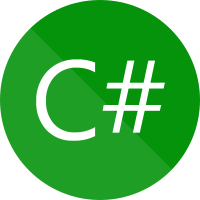
\includegraphics[width=2cm]{exercises/references/csharp.png}
\end{figure}

The following source code listing shows a program that prints the text \enquote{Hello LaTeX friends!} to the console. Like Java, C\# makes use of classes and main methods to build executable applications. 

\codeblock{csharp}{exercises/references/HelloLateXFriends.cs}




